\documentclass[11pt]{article}
\usepackage{ucs}
\usepackage{graphicx}
\usepackage[utf8x]{inputenc} 
\usepackage[russian]{babel}  
\usepackage{geometry}
\usepackage{epstopdf}

\geometry{left=2cm}
\geometry{right=1.5cm}
\geometry{top=2cm}
\geometry{bottom=2cm} 

\newcommand{\HRule}{\rule{\linewidth}{0.5mm}}

\newcommand\measurepage{\dimexpr\pagegoal-\pagetotal-\baselineskip\relax}

\newcommand\fillpage{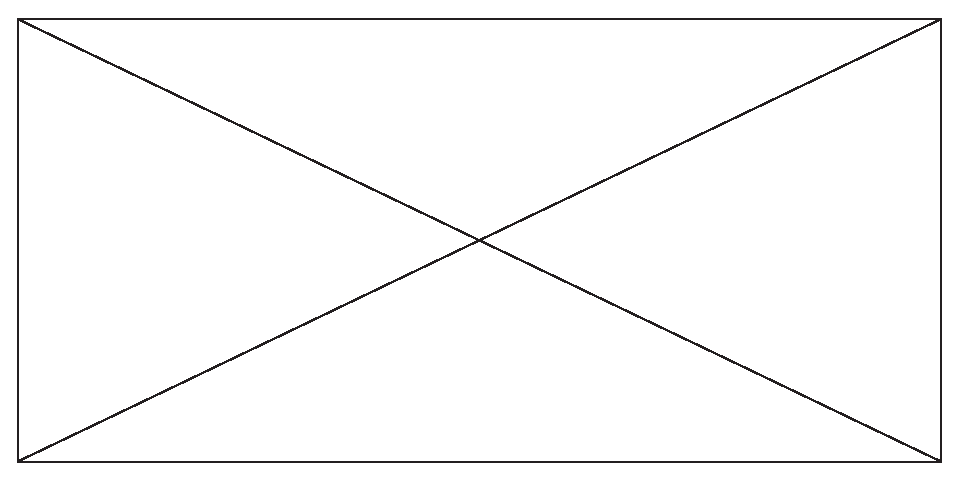
\includegraphics[width=\textwidth, height=\measurepage]{img/fill_page.eps}}

\begin{document}
   \begin{titlepage}
      \begin{center}
           \textsc{\LARGE{ФМЛ №30}}\\[1.5cm]
	\textsc{\Large Техническая документация}\\[0.5cm]
	{ \huge \bfseries Команда $\psi$ \\[0.4cm] }
	
\includegraphics[width=105mm,height=105mm]{img/icon.jpg}
      \end{center}
   \end{titlepage}
	\newpage
	
	\LARGE{Состав команды}
		\begin{table}[h]
			\begin{tabular}{|l|l|l|l|}
				\hline
				\textit{ФИО}         & Год рождения & Место учебы   & Роль в команде                      \\ \hline
				Жадковский Александр &  1998        & ФМЛ №30       & Капитан команды                     \\ \hline
				Лутошкин Роман       &  1998        & Гимназия №642 & Ответственный за техническую книгу, \\
				                     &              &               & оператор № 1                        \\ \hline
				Ильясов Александр    &  1999        & ФМЛ №30       & Оператор №2                         \\ \hline
				Поникаровский Антон  & 1998         & ФМЛ №30       & Запасной оператор                   \\ \hline
			\end{tabular}
		\end{table}
		\newpage
		
	\section{Описание робота}
		\subsection{Конструкция}
			\begin{itemize}
				\item Робот должен быть небольшим и мобильным
				\item Конструкция должна быть наиболее простой с максимально легким доступом ко всем узлам конструкции
				\item Робот должен обладать механизмом подъема, способным подниматься на высоту 120 см и выше
				\item По возможности робот должен обладать специальным приспособлением для зацепки корзин и их перемещения
			\end{itemize}
			\fillpage
			
		\subsection{Стратегия}
			Период выступления делится на 2(3) периода: автономный период и основное время, которое состоит из первых 1.5 минут и последних 30 секунд.
			В автономном периоде робот должен:
			\begin{itemize}
				\item В зависимости от расположения, съехать с пандуса или выехать вперед
				\item Сориентироваться согласно ИК-датчику и сбить подпорку корзины
				\item Захватить максимально возможное кол-во шариков(Но не более 5-ти)
			\end{itemize}
			После автономного периода следует управляемый двухминутный период в котором необходимо:
			\begin{itemize}
				\item Выгрузить захваченные в автономном периоде шарики в центр. корзину
				\item Захватить новые шарики 
				\item Повторять такую процедуру до окончания времени
				\item В конце вернуться на зону парковки
			\end{itemize}
			\fillpage
	
	\subsection{Материалы, использованные в роботе}

\begin{enumerate}
	\item Алюминиевая ось 1м х 8мм. 2 экз.
	\item Алюминиевый профиль 1м х 10мм х 10мм. 4 экз.
	\item Пластмасса ПЭТ листовая 20 см х 2 м. 1 экз.
	\item Оцинкованная сталь лист 1м х 1м х 1 мм. 1 экз.
	\item Мебельная рейка 35см. 2 экз.
	\item Леска.
	\item Термоклей.
	\item Изолента.
	\item Хомуты пластиковые
\end{enumerate}
\fillpage
\newpage
	
	\section{Основная часть}
	
	\subsection{16.09.14}
	
	\begin{enumerate}
		\item Дата собрания : 16.09.14
		\item Цель:
		\begin{itemize}
			\item Собрать основу робота, а именно колесную базу
			\item Написать простейшую программу для управления роботом
		\end{itemize}			
		\item Реализация :
		\begin{itemize}
			\item Была собрана квадратная конструкция(Рис. 1)
			\item Написана программа для передвижения
		\end{itemize}
		\item Результаты
		\begin{itemize}
			\item Собран четырехколесный робот, способный передвигаться по четырем направлениям
			\item Робот управляется с помощью геймпада
		\end{itemize}
		Получившаяся конструкция:
		\begin{figure} [h]
			\centering
			\begin{minipage}{0.3\linewidth}
				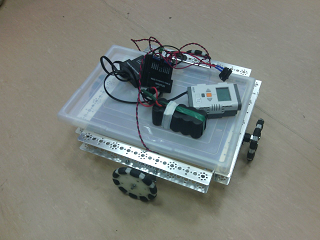
\includegraphics[width=35mm,height=35mm]{Days/16.09.14/1_1_robot.png}\\ Рисунок 1
			\end{minipage}
			\begin{minipage}{0.3\linewidth}
				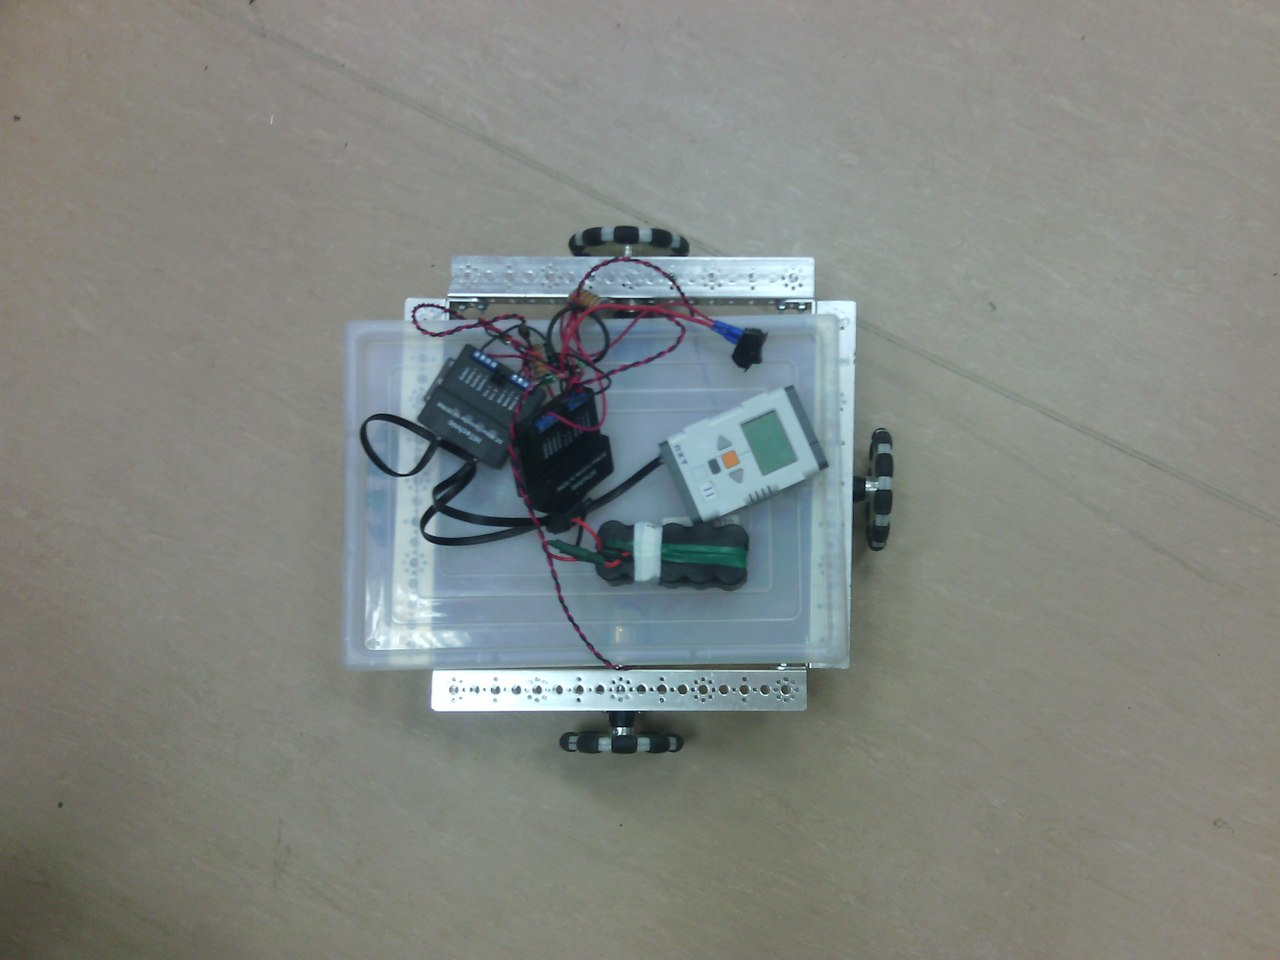
\includegraphics[width=35mm,height=35mm]{Days/16.09.14/1_2_robot}\\ Рисунок 2
			\end{minipage}
		\end{figure}
	\end{enumerate}
	
	\subsection{24.09.14}
	
	\begin{enumerate}
		\item Дата собрания : 24.09.14
		\item Цель:
		\begin{itemize}
			\item Перевернуть двигатели передвижения в креплениях для увеличения дорожного просвета.
			\item Укрепить и окончательно установить катушки для наматывания лески.
			\item Написать программу управления роботом с помощью стиков геймпада и протестировать движение робота, в том числе заезд и съезд с пандуса.
		\end{itemize}
		\item Результаты:
		\begin{itemize}
			\item Двигатели перевёрнуты, дорожный просвет увеличился примерно на 2 см.
			\item Катушки укреплены, барабан намотки увеличен, что позволяет наматывать леску с большей скоростью.
			\item Программа написана, робот заезжает на пандус достаточно долго и неуклюже.
			\item Немного изменена проводка, добавлена деталь, которой не хватало на прошлых занятиях – кнопка включения питания.
		\end{itemize}	
		\item Идеи:
		\begin{itemize}
			\item Заменить в подъёмнике рейки из набора TETRIX на алюминиевый профиль, соединить два подъёмника поперечными рейками, в т.ч. той, которую будет тянуть леска, намотать леску, проверить работу подъёмника.
			\item В будущем изменить колёсную базу, т.к. эта показывает плохие результаты при заезде на пандус.
		\end{itemize}
	\end{enumerate}


	\subsection{31.09.14}
	
  \begin{enumerate}
    \item Дата собрания : 31.09.14
    \item Цель:
    \begin{itemize}
      \item Установить мебельные рейки боком к земле для того, чтобы они выдерживали большую нагрузку. Мы не учли это при первоначальной сборке, в результате чего на первом отборочном туре в городе Сочи при усиленных тренировках на эти рейки, которые на тот момент были установлены параллельны земле, оказывалось крайне большое давление в неправильной плоскасти, что вызвало поломку этих мебельных реек(подвижная часть так сильно отогнулась от неподвижной, в результате чего из рейки вылетели все подшипники, обеспечивающие работу рейки). Мы осознали, что мебельные рейки в производстве используются немного подругому, то есть их устанавливают в другой плоскости. Представим тумбочку с выдвижными ящиками. Её движение обоеспечиваюдт мебельные рейки схожие с теми, что использовали мы, только в тумбочке они установлены перпендикулырно земле, что не приводит к отгибу подвижной части рейки от неподвижной.
      \item Разметить места для сверления балок для обеспечения свободного прохождения реек через отверстия в балках.
      \item Укрепить ось, через которую перекидывается леска, так как из-за большой нагрузки на эту ось она деформировалась(прогнулась).
    \end{itemize}
    \item Результаты:
    \begin{itemize}
      \item Мебельные рейки установлены боком. Теперь пространство между сторонами будущего подъёмника значительно увеличилось по сравнению с предыдущей версией робота за счёт того, что мы установили мебельные рейки на несущие балки(на основу конструкции). Таким образом пространство в роботе у нас сильно увеличилось, что способствует созданию большей корзины и механизма для захвата.
      \item Отверстия для реек размечены, отверстия пока не просверленны, так как для этого необходимо проводить довольно масштабную разборку робота.
      \item Ось, через которую перекидывается леска, укреплена - на неё надет алюминиевый профиль, что сделало её вомного раз более крепкой и устойчивой к прогибу.
    \end{itemize} 
    \item Идеи:
    \begin{itemize}
    	\item Основной план - продолжать переделывать робота, в частности начать изготавливать подъёмник из уже распиленных алюминиевых балок.
	\item Необходимо грамотно установить проводку на нашего робота таким образом, чтобы был доступен блок NXT, была легкодоступна кнопка включения и выключения, чтобы можно было оперативно заменить аккумулятор NXT и TETRIX или подзарядить его. Необходимо, чтобы все контроллеры были подключены параллельно, так как при поломке одного из контроллеров, подключенных последовательно, остальные перестанут питаться электричеством, что может привести к полной демобилизации нашего робота.
    	\item Также необходимо сделать ёмкость для захвата шариков с захватом для них, её планируется сделать из пластика, так как пластик наиболее пластичен и с ним удобно работать.
    \end{itemize}
   \end{enumerate}
\fillpage
		

	\subsection{3.10.14}
	
\begin{enumerate}
		\item Дата собрания 3.10.14
		\item Цель:
		\begin{itemize}
			\item Укрепить конструкцию робота
			\item Разнести колеса по углам конструкции для увеличения площади колесной базы
			\item Закрепить основные узлы управления робота на конструкции с максимально легким доступом к ним
			\item Оптимизировать программу, перенести управление передвижением робота с кнопок на джойстик
		\end{itemize}
		\item Результаты:
		\begin{itemize}
			\item Конструкция робота была укреплена, центр тяжести снижен 
			\item Двигатели были закреплены по углам конструкции, одновременно закрепляя ее
			\item На осях был закреплен второй ряд колес определенным образом для лучшего управления(Рисунок 2,3)
		\end{itemize}
		\begin{figure} [h]
			\centering
			\begin{minipage}{0.3\linewidth}
				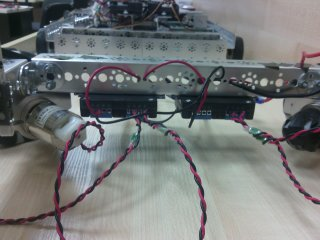
\includegraphics[width=35mm,height=35mm]{Days/3.10.14/3_1_robot}\\ Рисунок 3
			\end{minipage}
			\begin{minipage}{0.3\linewidth}
				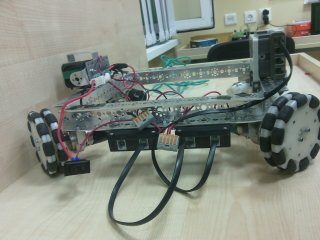
\includegraphics[width=35mm,height=35mm]{Days/3.10.14/3_2_robot}\\ Рисунок 4
			\end{minipage}
			\begin{minipage}{0.3\linewidth}
				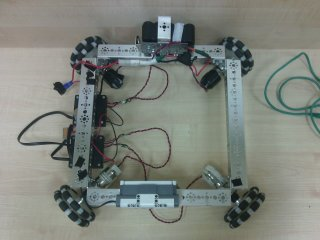
\includegraphics[width=35mm,height=35mm]{Days/3.10.14/3_3_robot}\\ Рисунок 5
			\end{minipage}
		\end{figure}
		\item Идеи и планы для следующего занятия:
		\begin{itemize}
			\item Начать строить механизм захвата и подъема шариков. В качесте механизма подъема можно использовать ножничный подъемник, механизм захвата еще обдумывается
		\end{itemize}
	\end{enumerate}
	\fillpage
\newpage
	
	\subsection{13.10.14}
	
	\begin{enumerate}
		\item Цель:
		\begin{itemize}
			\item Реализовать ножничный подъемник, механизм, приводящий его в движение и закрепление на кострукции робота
			\item Написать программу для управления захватом с отдельного геймпада
		\end{itemize}
		\item Результаты:
		\begin{itemize}
			\item Робот был частично разобран из-за недостатка деталей, была собрана примерная схема механизма передвижения подъемника(Рисунок 6)
			\item Написать и отладить программу не получилось, опять же из-за отсутствия деталей
			\item При тестировании барабана для намотки лески обнаружился очень сильный изгиб конструкции во время вращения барабана. Возможно, проблема в неоткалиброванном барабане или осях моторов, находящихся на разных уровнях. Попытаемся исправить это на следующем занятии.
		\end{itemize}
		\item Идеи:
		\begin{itemize}
			\item Заменить текущие рейки в подъемнике на алюминиевые профили для удобства установки, увеличения длины составляющих подъемника и уменьшения веса конструкции
			\item Отказаться от омниколес, поставить 4 обычных колеса
		\end{itemize}
		\item Рисунки:
		\begin{figure} [h]
			\centering
			\begin{minipage}{0.3\linewidth}
				\includegraphics[width=40mm,height=25mm]{Days/13.10.14/5_1_robot}\\ Рисунок 6
			\end{minipage}
			\begin{minipage}{0.3\linewidth}
				\includegraphics[width=40mm,height=25mm]{Days/13.10.14/5_2_robot}\\ Рисунок 7
			\end{minipage}
		\end{figure}
	\end{enumerate}
	\clearpage

	
	\subsection{15.10.14}
	
	\begin{enumerate}
	\item Дата собрания: 15.10.14
	\item Цель:
		\begin{itemize}
		\item Заменить омни-колеса на обычные
		\item Начать готовить профили для подъемника
		\item Решить проблему с барабаном
		\end{itemize}
	\item Результаты:
		\begin{itemize}
		\item Было установлено два колеса, оба ведущие. Так как теперь они установлены не в углах конструкции уменьшилась площадь опорной поверхности $\Rightarrow$ уменьшилась стабильность робота.
		\item Профили были распилены на отдельные части определенного размера и пропилены отверстия для креплений
		\item Проблема не была решена, вся конструкция ходит туда-сюда по-прежнему. Было решено оставить этот элемент в покое на данный момент времени и заняться колесной базой.
		\end{itemize}
	\item Идеи и планы:
		\begin{itemize}
		\item Установить оставшиеся колеса и испытать робота на поле
		\item Начать строить подъемник
		\end{itemize}
		\begin{figure} [h]
			\centering
			\begin{minipage}{0.3\linewidth}
				\includegraphics[width=35mm,height=35mm]{Days/15.10.14/8_1_robot}\\ Рисунок 8
			\end{minipage}
		\end{figure}
	\end{enumerate}
\fillpage
\newpage


	
	\subsection{17.10.14}
	
	\begin{enumerate}
	\item Дата собрания: 17.10.14
	\item Цель:
		\begin{itemize}
		\item Установить оставшиеся колеса, проверить подвижность робота(способность разворачиваться, заезжать на пандус и спускаться с него)
		\item Придумать(по возможности установить) конструкцию подъемника
		\end{itemize}
	\item Результаты:
		\begin{itemize}
		\item Проведя несколько пробных заездов с уже собранной конструкцией выяснилось, что робт имеет недостаточное сцепление с полем. Было решено заменить текущую колесную базу на трехколесную.
		\item Подходящих креплений для установки подъемника не нашлось. Крепления должны прочно, без люфтов, скреплять балочные элементы подъемника, при этом не создавая большого трения между ними.
		\item Для уменьшения люфтов и трения в основании конструкции были установлены выдвижные рейки(Рисунки 8, 9)
		\end{itemize}
	\item Идеи и планы:
		\begin{itemize}
		\item Установть вместо двух опорных омни-колес одно
		\item Появилась идея использовать в качестве креплений для подъемника мебельные стяжки.
		\end{itemize}
	\begin{figure} [h]
			\centering
			\begin{minipage}{0.3\linewidth}
				\includegraphics[width=35mm,height=35mm]{/!my_data/projects/pml30-psi_team/Days/17.10.14/7_1_robot}\\ Рисунок 8
			\end{minipage}
			\begin{minipage}{0.3\linewidth}
				\includegraphics[width=35mm,height=35mm]{/!my_data/projects/pml30-psi_team/Days/17.10.14/7_2_robot}\\ Рисунок 9
			\end{minipage}
			\begin{minipage}{0.3\linewidth}
				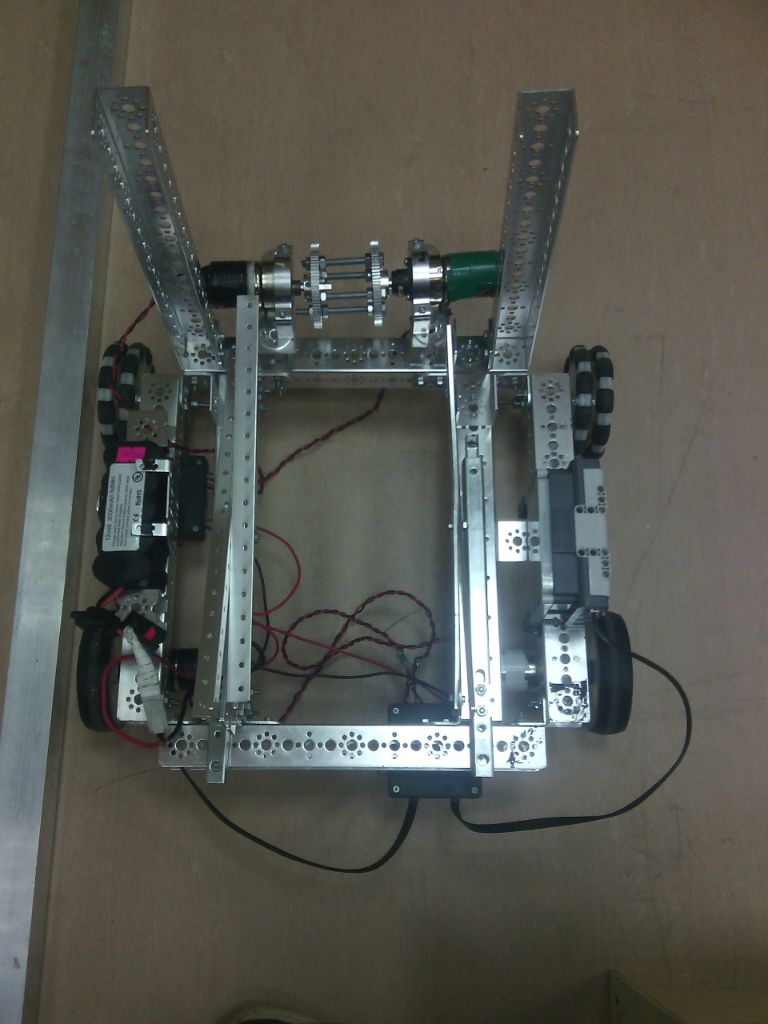
\includegraphics[width=35mm,height=35mm]{/!my_data/projects/pml30-psi_team/Days/17.10.14/7_3_robot}\\ Рисунок 10
			\end{minipage}		
	\end{figure}
	\end{enumerate}
\newpage

	\subsection{24.10.14}
	
	\begin{enumerate}
		\item Дата собрания: 24.10.14
		\item Цель:
		\begin{itemize}
			\item Установить одно опорное колесо вместо двух
			\item Попробовать мебельные стяжки в качестве креплений балочных элементов подъемника
			\item Проверить подвижность робота
		\end{itemize}			
		\item Результаты:
		\begin{itemize}
			\item Приводные колеса робота были отодвинуты назад примерно на 5см, так как робот очень часто вставал на задние колеса и переворачивался
			\item Стяжки хорошо проявили себя в качестве креплений: они не создают почти никакого трения, при этом сохраняя стабильность конструкции
			\item Робот оказался довольно подвижным, забирается на пандус, разворачивается на нем и спускается без проблем
			\item Программа была написана для максимально легкого управления
		\end{itemize}
		\item Идеи и планы:
		\begin{itemize}
			\item Оставить колесную базу в покое и начать строить только подъемник
		\end{itemize}
		\begin{figure} [h]
			\centering
			\begin{minipage}{0.3\linewidth}
				\includegraphics[width=35mm,height=35mm]{/!my_data/projects/pml30-psi_team/Days/24.10.14/9_1_robot}\\ Рисунок 11
			\end{minipage}
			\begin{minipage}{0.3\linewidth}
				\includegraphics[width=35mm,height=35mm]{/!my_data/projects/pml30-psi_team/Days/24.10.14/10_2_robot}\\ Рисунок 12
			\end{minipage}
			\begin{minipage}{0.3\linewidth}
				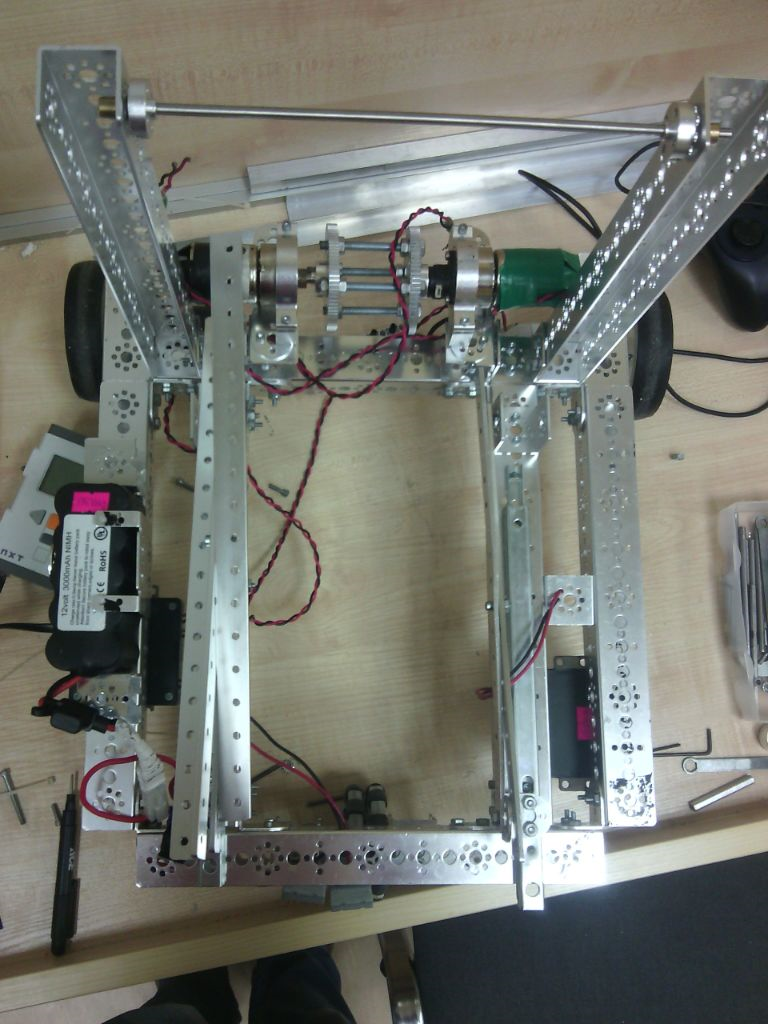
\includegraphics[width=35mm,height=35mm]{/!my_data/projects/pml30-psi_team/Days/24.10.14/9_4_robot}\\ Рисунок 13
			\end{minipage}
		\end{figure}
	\end{enumerate}
\newpage	
	
	\subsection{5.11.14}
	
	\begin{enumerate}
		\item Дата собрания: 5.11.14
		\item Цель:
		\begin{itemize}
			\item Полностью собрать подъемник и испытать его
			\item Написать программу для управления им
		\end{itemize}			
		\item Реализация:
		\begin{itemize}
			\item Подъемник был собран, под стяжки пришлось расширить уже просверленые отверстия
			\item Механизм передвижения подъемника был переделан на более простой.
		\end{itemize}
		\item Результаты:
		\begin{itemize}
			\item Шестеренки при подъеме конструкции соскальзывали из-за слишком большого усилия, оси слышком сильно выгибались по той же причине.
		\end{itemize}
		\item Идеи и планы:
		\begin{itemize}
			\item Поставить меньшее передаточное отношение
			\item Установить более прочные оси
		\end{itemize}
		\begin{figure} [h]
			\centering
			\begin{minipage}{0.3\linewidth}
				\includegraphics[width=35mm,height=35mm]{Days/5.11.14/10_1_robot}\\ Рисунок 14
			\end{minipage}
			\begin{minipage}{0.3\linewidth}
				\includegraphics[width=35mm,height=35mm]{Days/5.11.14/10_3_robot}\\ Рисунок 15
			\end{minipage}
		\end{figure}
	\end{enumerate}
\newpage	

	\subsection{10.11.14}
		\begin{enumerate}
	\item Цель:
		\begin{itemize}
			\item Найти и поставить более прочные оси, способные выдерживать подобную нагрузку
			\item Усилить механизм передвижения подъемника
			\item Сделать конструкцию подъемника более стабильной
		\end{itemize}
	\item Реализация: 
		\begin{itemize}
			\item Программа была написана для второго оператора, управление высотой подъема происходит через джойстик, в будущем будет установлен резервуар для временного хранения шариков, который будет открываться/закрываться при помощи сервопривода по команде оператора.
			\item Устойчивость подъемника была увеличена путем установки второй оси, соединяющий две стороны подъемника. На самом верху конструкции были установлены еще две выдвижные рейки, повышающие стабильность конструкции и позволяющие с большей легкостью установить резервуар.(Рисунки 16, 17)
			\item Исправить слишком сильное выгибание оси под нагрузкой удалось путем жесткого закрепления оси на специальных креплениях, установленных на конструкции робота.(Рисунок 18)
			\begin{minipage}{0.3\linewidth}
			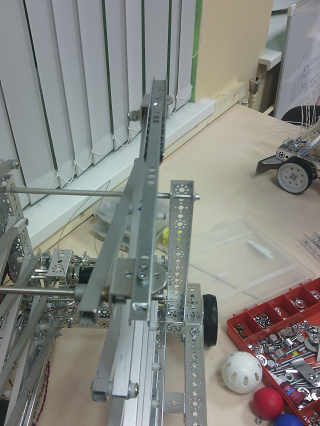
\includegraphics[width=45mm,height=45mm]{Days/10.11.14/11_1_robot}\\ Рисунок 16
			\end{minipage}
			\begin{minipage}{0.3\linewidth}
			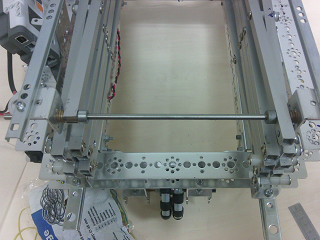
\includegraphics[width=45mm,height=45mm]{Days/10.11.14/11_2_robot}\\ Рисунок 17
			\end{minipage}
			\begin{minipage}{0.3\linewidth}
			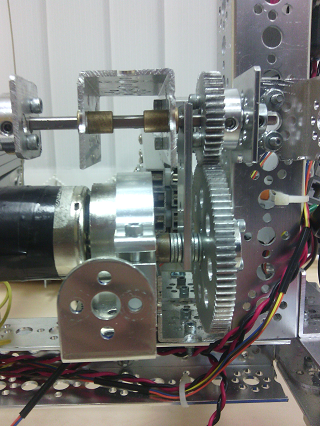
\includegraphics[width=45mm,height=45mm]{Days/10.11.14/11_4_robot}\\ Рисунок 18
			\end{minipage}
		\end{itemize}
		\newpage
		\item Идеи и планы:
			\begin{itemize}
				\item Доделать резервуар и установить на него сервопривод
				\item Попытаться сделать что-либо для возвращения подъемника в изначальное - сложенное - состояние, так как под собственным весом он этого сделать не может.
			\end{itemize}
\end{enumerate}
\fillpage

	
	\subsection{15.11.14}
	\begin{enumerate}
	\item Цель:
		\begin{itemize}
			\item Сделать резервуар, способный вместить в себе 5 больших шариков, оснастить его сервоприводом со стенкой, закрывающим резервуар и установить на робота.
			\item Придумать способ возвращения конструкции в изначальное положение.
			\item Написать программу для управления сервоприводом 
		\end{itemize}
	\item Реализация:
		\begin{itemize}
			\item Резервуар был сделан при помощи железной сетки и пластиковой вазы. При установке выяснилось, что контейнер слишком широкий и слишком сильно трется о внутреннюю поверхность подъемника. (Рисунки 21, 22)
			\item В качестве возвращающего механизма были использованы обычные канцелярские резинки(Рисунки19, 20)\\
			\begin{minipage}{0.3\linewidth}
			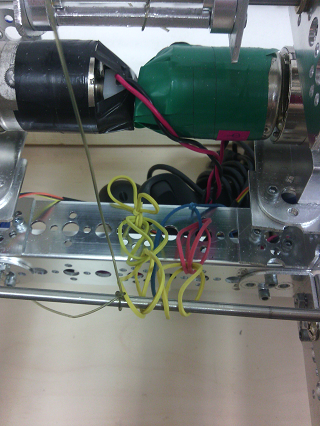
\includegraphics[width=45mm,height=45mm]{Days/15.11.14/12_1_robot}\\ Рисунок 19
			\end{minipage}
			\begin{minipage}{0.3\linewidth}
			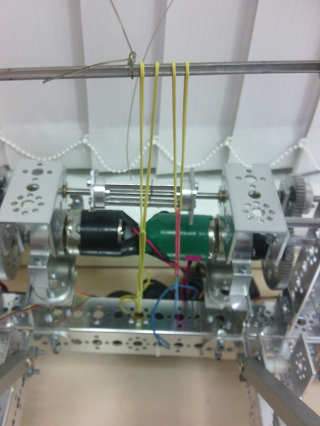
\includegraphics[width=45mm,height=45mm]{Days/15.11.14/12_2_robot}\\ Рисунок 20
			\end{minipage}\\
			\begin{minipage}{0.3\linewidth}
			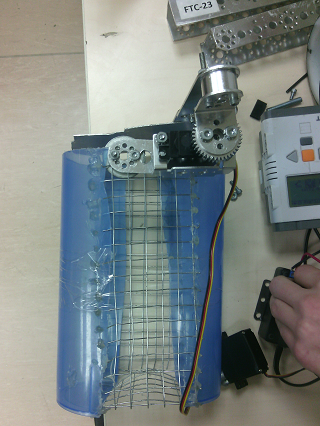
\includegraphics[width=45mm,height=45mm]{Days/15.11.14/12_3_robot}\\ Рисунок 21
			\end{minipage}
			\begin{minipage}{0.3\linewidth}
			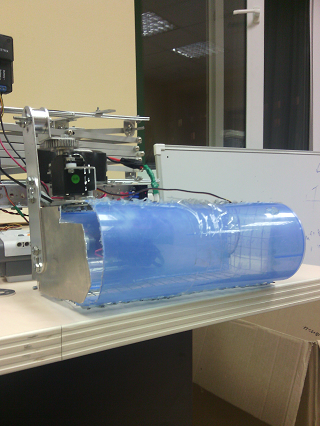
\includegraphics[width=45mm,height=45mm]{Days/15.11.14/12_4_robot}\\ Рисунок 22
			\end{minipage}\\
		\end{itemize}
	\item Идеи и планы:
		\begin{itemize}
			\item Закрепить резервуар на конструкции все же не удалось. На следующем занятии планируем сделать новый, меньшего размера и другой формы, закрпеить его на конструкции и протестировать.
			\item Тренироваться.
		\end{itemize}
		\fillpage
\end{enumerate}

	\subsection{Соревнования "Робофест-Юг" 21-14 ноября }
	\begin{center}
	
\includegraphics{Days/21-24.11.14/robofest_logo.png}
\end{center}
С 21 по 24 ноября 2014 года наша команда впервые выступила на соревновании - Робофест-Юг. Это была возможность посмотреть на настоящие соревнования в категории FTC, проверить робота в экстремальных условиях, пообщаться с другими командами и, по возможности, выиграть.\\
Согласно изначальной задумке, наш робот должен был в автономном периоде съезжать с горки, подъезжать к автономной корзине и закидывать туда автономные мячи. Так как к соревнованиям робот был готов не полностью, нам пришлось переделывать его конструкцию так как:
\begin{itemize}
	\item Корзина для захвата мячей не влезала в проем между сторонами подъемника и он не мог подниматься;
	\item В автономном периоде робот мог только съезжать с пандуса.
	\item Из-за повышающей передачи конструкция сильно прогибалась под нагрузкой.
\end{itemize}
После устранения проблемы с проводкой, мы пошли на тренировочное поле, чтобы посмотреть на поведение робота на поле. Робот довольно неплохо управлялся, спокойно заезжал на пандус и спускался с него и без проблем выбивал подпорку для контейнера с шариками. Выяснились как хорошие, так и плохие стороны робота. Выяснилось, что робот очень хорошо приспособлен к перемещению мензурок по полю, в том числе затаскивания их на пандус. С другой стороны, робот не мог забросить мяч ни в одну корзину, так как захватывать мячи в корзину с такой конструкцией было практически невозможно, они постоянно вываливались и сама корзина очень сильно шаталась, укрепление конструкции не спасло. На время соревнований было решено заменить корзину на клешню, способную захватить только один мяч. \\
После некоторого количества тренировок порвалась леска, поднимающая конструкцию. Буквально сразу после ее замены, при первом же испытании, она снова порвалась. Просмотрев всю конструкцию на наличие дефектов, мы ничего не нашли. На третий раз был слышен характерный треск. выяснилось, что сломались пополам две нижние балки и выломана рейка. Причина поломки была выяснена позднее - одно из креплений было перезатянуто и не давало подъемнику раскладываться без проблем. \\
	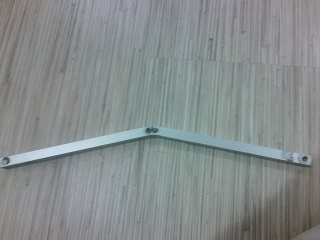
\includegraphics{Days/21-24.11.14/11_1_robot.png}
	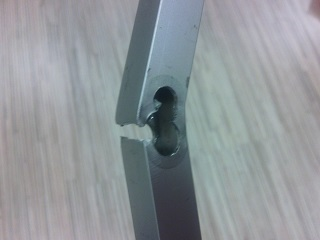
\includegraphics{Days/21-24.11.14/11_2_robot.png}\\
\emph{Вот так выглядела балка после поломки}.\\
Так как починить и отладить подъемник времени не было, мы решили просто удалить нижнюю секцию, уменьшив тем самым высоту подъема примерно до 90 см. Было принято решение сосредоточиться на выбивании подпорки и передвижении мензурок по полю, а в последние 30 секунд на заезде на пандус с мензуркой.\\
В таком темпе проходила квалификация, параллельно мы пытались ловить клешней шарики, но из-за раскачивания клешни и отсутствия ограниченного сервопривода, способного удерживать клешню в одном положении, ничего не выходило.\\
На следующий день подводились итоги квалификации.\\
	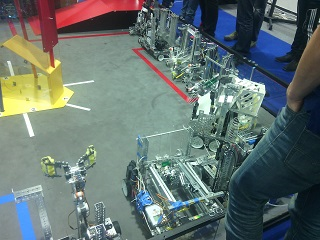
\includegraphics{Days/21-24.11.14/11_3_robot.png}
	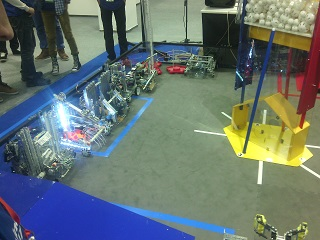
\includegraphics{Days/21-24.11.14/11_4_robot.png}\\
	\emph{Показ всех роботов для отбора в финал}.\\
 Наш робот не вышел в топ-5 по матч-поинтам и не был выбран в финальную битву. На этом наше участие в соревновании кончилось. Для себя мы выяснили, что нужно больше взаимодействовать с другими командами и заранее все рассчитывать.
В планах у нас было тотальное изменение конструкции робота:
\begin{itemize}
	\item Увеличение ширины подъемника для более легкой установки корзины
	\item Трехколесная база не проявила себя, поэтому было принято решение вернуться к четырехколесной
	\item Переделать балки подъемника, так как текущие сделаны с очень большой погрешностью. 
\end{itemize}
\fillpage
	
	\subsection{5.12.14}
	
  \begin{enumerate}
    \item Дата собрания : 24.09.14
    \item Цель:
    \begin{itemize}
      \item Установить мебельные рейки боком к земле для того, чтобы они выдерживали большую нагрузку. Мы не учли это при первоначальной сборке, в результате чего на первом отборочном туре в городе Сочи при усиленных тренировках на эти рейки, которые на тот момент были установлены параллельны земле, оказывалось крайне большое давление в неправильной плоскасти, что вызвало поломку этих мебельных реек(подвижная часть так сильно отогнулась от неподвижной, в результате чего из рейки вылетели все подшипники, обеспечивающие работу рейки). Мы осознали, что мебельные рейки в производстве используются немного подругому, то есть их устанавливают в другой плоскости. Представим тумбочку с выдвижными ящиками. Её движение обоеспечиваюдт мебельные рейки схожие с теми, что использовали мы, только в тумбочке они установлены перпендикулырно земле, что не приводит к отгибу подвижной части рейки от неподвижной.
      \item Разметить места для сверления балок для обеспечения свободного прохождения реек через отверстия в балках.
      \item Укрепить ось, через которую перекидывается леска, так как из-за большой нагрузки на эту ось она деформировалась(прогнулась).
    \end{itemize}
    \item Результаты:
    \begin{itemize}
      \item Мебельные рейки установлены боком. Теперь пространство между сторонами будущего подъёмника значительно увеличилось по сравнению с предыдущей версией робота за счёт того, что мы установили мебельные рейки на несущие балки(на основу конструкции). Таким образом пространство в роботе у нас сильно увеличилось, что способствует созданию большей корзины и механизма для захвата.
      \item Отверстия для реек размечены, отверстия пока не просверленны, так как для этого необходимо проводить довольно масштабную разборку робота.
      \item Ось, через которую перекидывается леска, укреплена - на неё надет алюминиевый профиль, что сделало её вомного раз более крепкой и устойчивой к прогибу.
    \end{itemize} 
    \item Идеи:
    \begin{itemize}
    	\item Основной план - продолжать переделывать робота, в частности начать изготавливать подъёмник из уже распиленных алюминиевых балок.
	\item Необходимо грамотно установить проводку на нашего робота таким образом, чтобы был доступен блок NXT, была легкодоступна кнопка включения и выключения, чтобы можно было оперативно заменить аккумулятор NXT и TETRIX или подзарядить его. Необходимо, чтобы все контроллеры были подключены параллельно, так как при поломке одного из контроллеров, подключенных последовательно, остальные перестанут питаться электричеством, что может привести к полной демобилизации нашего робота.
    	\item Также необходимо сделать ёмкость для захвата шариков с захватом для них, её планируется сделать из пластика, так как пластик наиболее пластичен и с ним удобно работать.
    \end{itemize}
   \end{enumerate} \fillpage
	
	\subsection{8.12.14}
	
  \begin{enumerate}
    \item Дата собрания : 8.12.14
  	\item Цель:
  	\begin{itemize}
  	  \item Разработать концепцию дальнейшего построения робота, а также план её реализации. Разделить задачи на всех членов команды.
  	  \item Закрепить на корпусе робота всю необходимую электронику.
  	\end{itemize}
  	\item Результаты:
  	\begin{itemize}
  	  \item Направление дальнейшей работы над роботом выбрано, задачи распределены по всем членам команды.
  	  \item На корпусе робота размещена вся необходимая электроника так, чтобы она не мешала работе механизмов робота.
   	\end{itemize} 
   	\item Идеи:
   	\begin{itemize}
   		\item Рассверлить балки для подъёмника, собрать из них подъёмник, установить его.
   		\item Согнуть из листового пластика коробку для захвата шариков, собрать механизм для её переворота с помощью одного или двух ограниченных сервоприводов, закрепить всё это на верхней площадке подъёмника.
   		\item Протестировать работу робота в целом и всех механизмов в частности.
   	\end{itemize}
   \end{enumerate}
\fillpage

\end{document}
